\chapter{Conceptual study}
\lhead{\textit{Chapter \thechapter}}
\rhead{\textit{Conceptual study}}

\section{introduction}
This chapter describes a very important part which is the conceptual study and an analytical look in addition to the base design.\\
This part define the basic steps for developing our system where specifying functional and non-functional requirements using the concepts of Unified Modeling Language ( Use Case diagram, Sequence diagrams, and Class diagram), and clarify the goal of
this analysis and design all about the topic of computer architecture in the form of an interactive course.

\section{Graphic design }

\subsection{Modeling}
Modeling uses graphic notation to create visual models of software systems, the use of diagrams and illustrations makes something
complex more understandable, that's why Unified Modeling language (UML) \cite{Techopedia-UML} is a standardized modeling language enabling developers to specify, visualize, construct and document artifacts of a software system.\\
Thus, UML makes these artifacts scalable, secure and robust in execution. It is an important aspect involved in object-oriented software development.

\subsection{Definition of Unified Modeling language}
The Unified Modeling Language (UML) is a general-purpose, developmental, modeling language in the field of software engineering that is intended to provide a standard way to visualize the design of a system.\cite{YThi-UML}\\

The creation of UML was originally motivated by the desire to standardize the disparate notational systems and approaches to software design. It was developed at Rational Software in 1994–1995, with further development led by them through 1996.\cite{YThi-UML}\\

In 1997, UML was adopted as a standard by the Object Management Group (OMG), and has been managed by this organization ever since. In 2005, UML was also published by the International Organization for Standardization (ISO) as an approved ISO standard. Since then the standard has been periodically revised to cover the latest revision of UML. In software engineering, most practitioners do not use UML, but instead produce informal hand drawn diagrams; these diagrams, however, often include elements from UML.\cite{YThi-UML}




\section{Specification and needs analysis}

\subsection{Basic functions of the application}
The main requirements which are specifically related to the behavior and functions of the system can be summarized in the following points :
\begin{enumerate}
	\item Interactive course with practical examples.
	\item Fun Quiz and testing what the user has learned.
	\item Practical models for machine structure tests.
\end{enumerate} 
\subsection{Non-functional needs}
These are the most important major requirements not specifically related to the behavior of the system but rather the identification of internal and external constraints of the system :
\subsubsection{Ergonomic interfaces}
the solution must present an ergonomic interface encompassing all the functionalities. The manipulation of the interface should not require advanced computer knowledge, it must be simple and clear in order to adapt to the computer knowledge of the users.
\subsubsection{Reliability and speed}
The system must guarantee the speed and reliability of the search for information, as well as optimal management of resources.
\subsubsection{The code}
Must be clear to allow future evolutions or improvements.






\section{Detailed design}

\subsection{Use Case diagram}
Use Case Diagram describes functionality of a system in terms of actors, goals as use cases and dependencies among the use cases.\cite{Techopedia-UML}
\subsubsection{System}
Interactive Course For Structure Machine 1.
\subsubsection{Actors}
Specify a role played by a user or any other system interacting with the subject.\cite{Techopedia-UML}
\subsubsection{Use cases}
describes functionalities of the system .In this system :
\begin{enumerate}
	\item COURSE : When user click on COURSE he can see the hole CHAPTERS of the course, when he click on try in each TITLE of CHAPTERS a question window will apear with a specific type of question depends on the chapter's TITLE.
	\item QUIZ : When user click on QUIZ he can test what he learned in this course with a specific Options (choose chapters and number of questions), when clicking on start a question window will apear.
	\item TEST : When user click on TEST he will find a practical models for machine structure tests including the whole course.
\end{enumerate}

\subsubsection{Relations}
\begin{enumerate}
	\item INCLUDE : (QUIZ and Options),(Options and Question),(TEST and Question).
	\item EXTENTION : the rest of use cases.
\end{enumerate}

The figure \ref{fig:UseCaseD} represents this system's Use Case Diagram.

\newpage
%***************************************************
\begin{figure*}[ht]
	\centering
	\label{}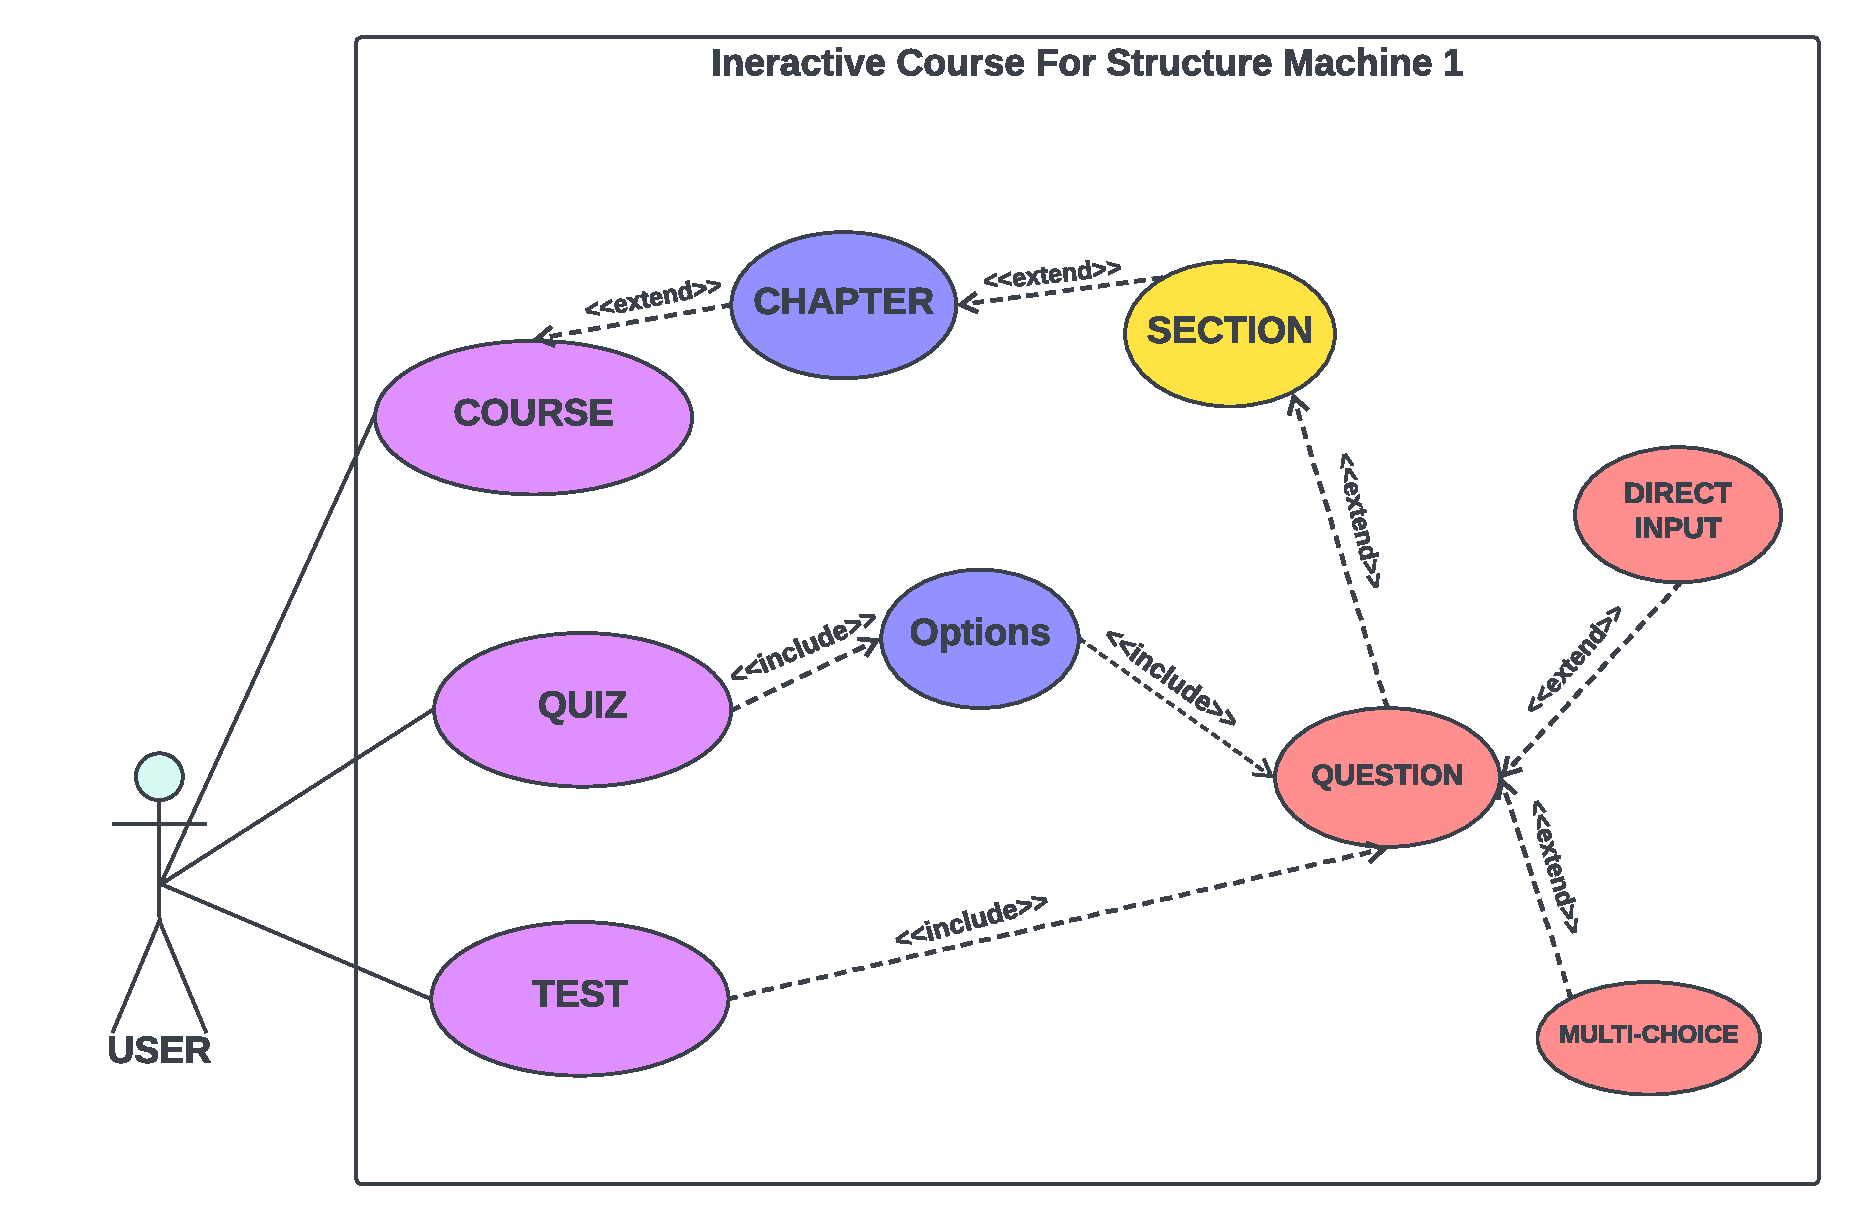
\includegraphics[scale=0.5]{img/Use Case.pdf}                
	\caption{Use Case diagram.} 
	\label{fig:UseCaseD}
\end{figure*} 
%===================================================================

\subsection{Sequence diagrams}
A sequence diagram, in the context of UML, represents object collaboration and is used to define event sequences between objects for a certain outcome, it is an essential component used in processes related to analysis, design and documentation.\cite{Techopedia-DS} \\\\
A sequence diagram is also known as a timing diagram, event diagram and event scenario.\cite{Techopedia-DS}

\subsection{COURSE}
This first scenario shows how user can see the hole CHAPTERS of the course, and try  a question with a specific type depends on the chapter's TITLE.

\newpage

\begin{table}[h!]
	\begin{center}
		\begin{tabular}{ |p{3cm}|p{9cm}|  }
 		\hline
 		\multicolumn{2}{|c|}{Identication summary} \\
 		\hline
 		Use Case Title & COURSE. \\
 		\hline
 		Abstract   & User learn course. \\
		\hline
 		Actor&  User. \\
		\hline
		\multicolumn{2}{|c|}{Identication summary} \\
		\hline
		Preconditions & Accessible system.  \\
		\hline
		User exists    &  The purpose of this system is navigate and learn from the course. \\
		\hline
		Scenario &  1- User clicks on Course button. \\ & 2- System loads all chapters. \\ & 3- System shows the chapters. \\ & 4- User chooses chapter. \\ & 5- System loads sections of chapter. \\ & 6- System shows the content of sections. \\ & 7- User clicks on Try. \\ & 8- System sends SQL request (Select section's question) to DataBase.\\ & 9- Database return data(section's question).\\ & 10- System loads results.\\ & 11- System shows results.\\
		\hline
		Object& User learn the course with live examples.   \\
 		\hline
\end{tabular}
\end{center}
\caption{Text Description of Use Case "COURSE".}
\label{tab:DS COURSE}
\end{table}



\newpage
The figure \ref{fig:COURSE DS} represents COURSE Sequence diagram.
%***************************************************
\begin{figure*}[ht]
	\centering
	\label{}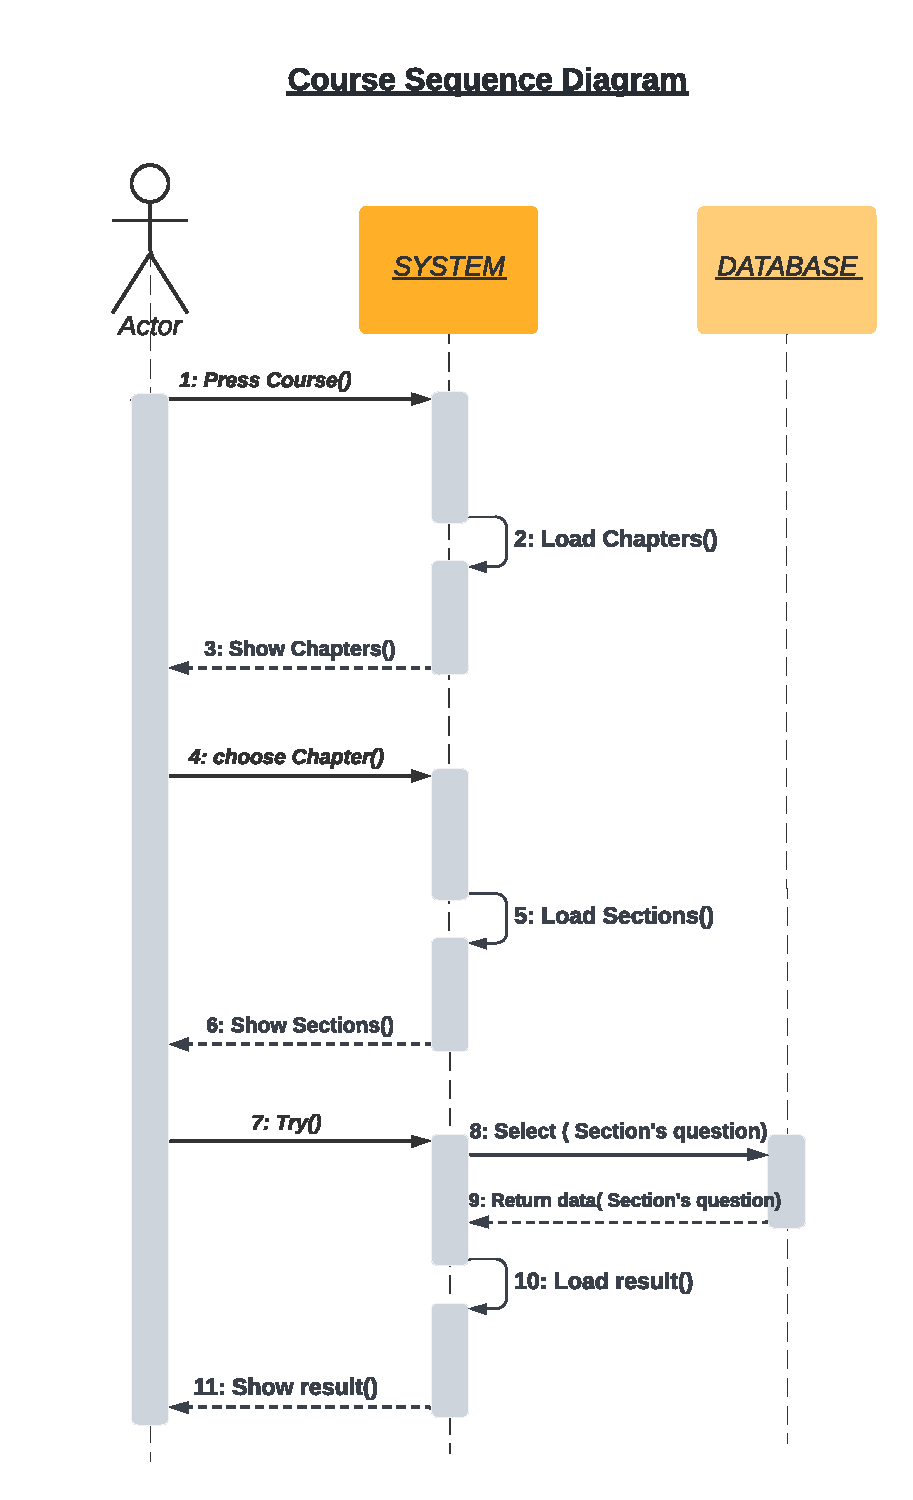
\includegraphics[scale=0.6]{img/Course Sequence diagram.pdf}                
	\caption{COURSE Sequence diagram.} 
	\label{fig:COURSE DS}
\end{figure*} 
%===================================================================






\subsection{QUIZ}
This second scenario shows how user can test what he learned in this course with a specific options (choose chapters and number of questions).
\newpage

\begin{table}[h!]
	\begin{center}
		\begin{tabular}{ |p{3cm}|p{9cm}|  }
			\hline
			\multicolumn{2}{|c|}{Identication summary} \\
			\hline
			Use Case Title & QUIZ. \\
			\hline
			Abstract   & User takes a quiz. \\
		   \hline
			Actor&  User. \\
		   \hline
		   \multicolumn{2}{|c|}{Identication summary} \\
		   \hline
		   Preconditions & Accessible system.  \\
		   \hline
		   User exists    &  The purpose of this system is taking a quiz. \\
		   \hline
		   Scenario &  1- User clicks on Quiz button. \\ & 2- System loads Options. \\ & 3- System shows Options. \\ & 4- User chooses options. \\ & 5- System shows Start button. \\ & 6- User clicks on Start button. \\ & 7- System sends SQL request (Select Questions) to DataBase. \\ & 8- Database return data(Questions).\\ & 9- System loads Quiz results.\\ & 10- System shows Quiz results.\\
		   \hline
		   Object&  User can take a quiz with any options he wants.  \\
			\hline
\end{tabular}
\end{center}
\caption{Text Description of Use Case "QUIZ".}
\label{tab:DS QUIZ}
\end{table}



\newpage
The figure \ref{fig:QUIZ DS} represents QUIZ Sequence diagram.
%***************************************************
\begin{figure*}[ht]
	\centering
	\label{}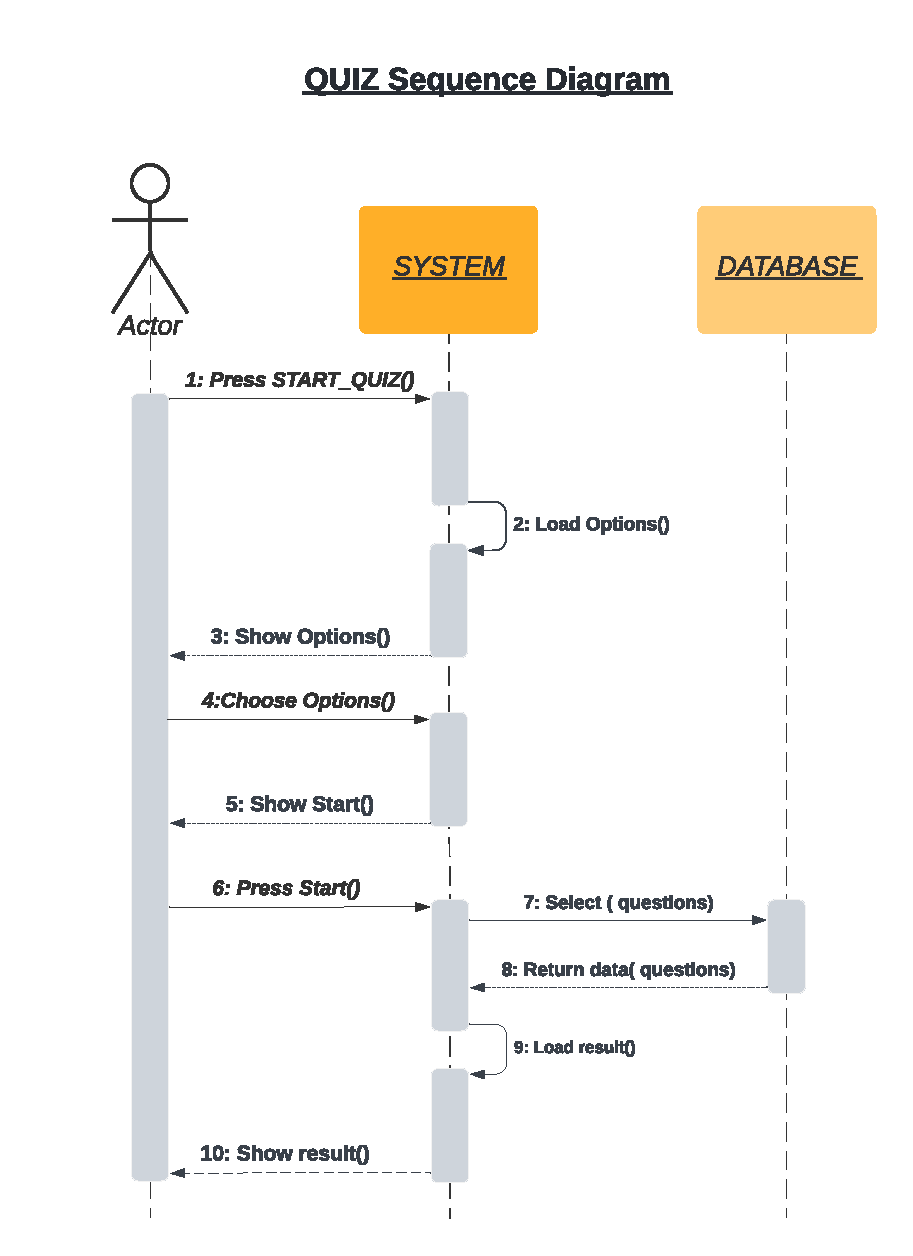
\includegraphics[scale=0.7]{img/Quiz Sequence diagram.pdf}                
	\caption{QUIZ Sequence diagram.} 
	\label{fig:QUIZ DS}
\end{figure*} 
%===================================================================







\subsection{TEST}
This third scenario shows how user can find a practical models for machine structure tests including the whole course.
\newpage

\begin{table}[h!]
	\begin{center}
		\begin{tabular}{ |p{3cm}|p{9cm}|  }
			\hline
			\multicolumn{2}{|c|}{Identication summary} \\
			\hline
			Use Case Title & Test. \\
			\hline
			Abstract   & User takes a Test. \\
		   \hline
			Actor&  User. \\
		   \hline
		   \multicolumn{2}{|c|}{Identication summary} \\
		   \hline
		   Preconditions & Accessible system.  \\
		   \hline
		   User exists    &  The purpose of this system is taking a Test. \\
		   \hline
		   Scenario &  1- User clicks on Test button. \\ & 2- System shows Start button. \\ & 3- User clicks on Start button. \\ & 4- System sends SQL request (Select Question from each chapter) to DataBase. \\ & 5- Database return data(Question from each chapter).\\ & 6- System loads Test results.\\ & 7- System shows Test results.\\
		   \hline
		   Object&  User can find a practical models for machine structure tests including the hole course. \\
			\hline
\end{tabular}
\end{center}
\caption{Text Description of Use Case "TEST".}
\label{tab:DS TEST}
\end{table}



\newpage
The figure \ref{fig:TEST DS} represents TEST Sequence diagram.
%***************************************************
\begin{figure*}[ht]
	\centering
	\label{}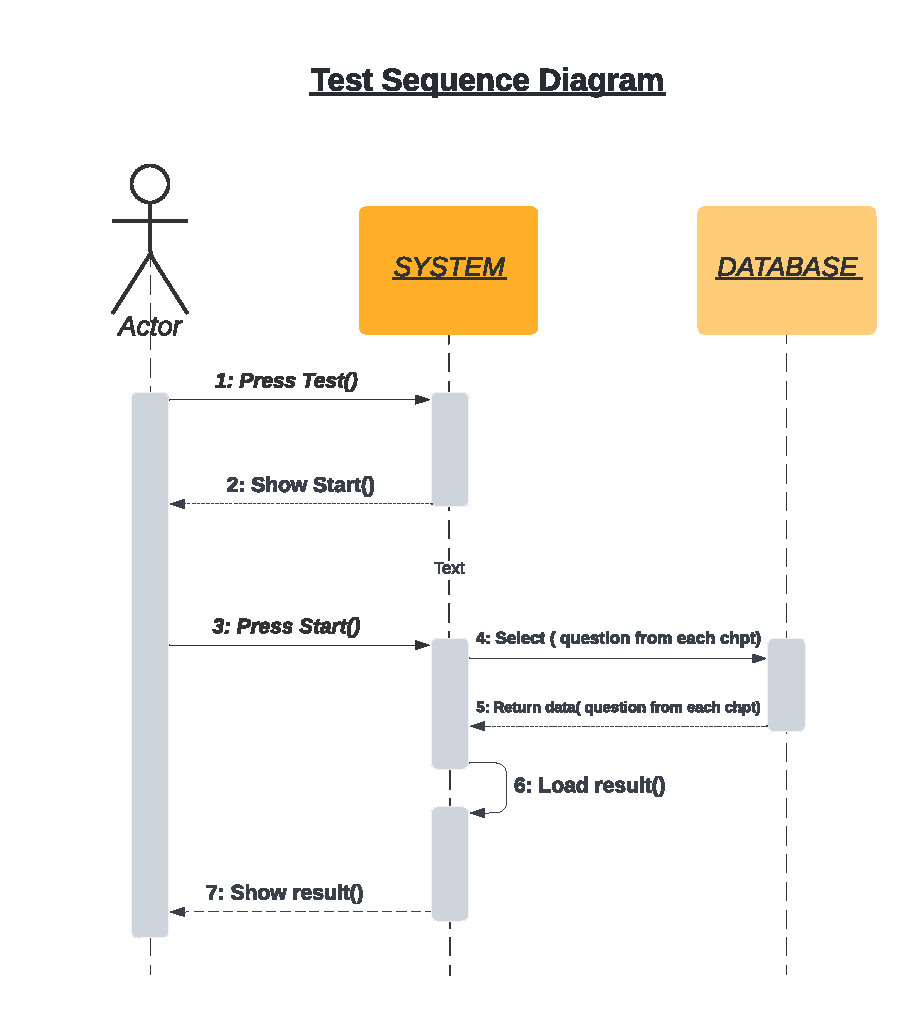
\includegraphics[scale=0.7]{img/Test Sequence diagram.pdf}                
	\caption{TEST Sequence diagram.} 
	\label{fig:TEST DS}
\end{figure*} 
%===================================================================




\subsection{Class Diagram}
A class diagram is a type of diagram and part of a unified modeling language (UML) that defines and provides the overview and structure of a system in terms of classes, attributes and methods, and the relationships between different classes. \cite{Techopedia-DC} \\
It is used to illustrate and create a functional diagram of the system classes and serves as a system development resource within the software development life cycle. \cite{Techopedia-DC} \\
\newpage

\subsubsection{Why Class Diagram?}
A class diagram is primarily designed for developers to provide the conceptual model and architecture of the system being developed. Typically, a class diagram consists of more than one class or all the created classes for a system. \cite{Techopedia-DC} \\
It is a type of structure diagram and looks similar to a flow chart having three main parts illustrated in rectangular boxes. The first or top part specifies the class name, the second or middle specifies attributes of that class and the third or bottom section lists the methods or operations that specific class can perform. \cite{Techopedia-DC} \\

The figure \ref{fig:DC} represents this system's Class Diagram.


%***************************************************
\begin{figure*}[ht]
	\centering
	\label{}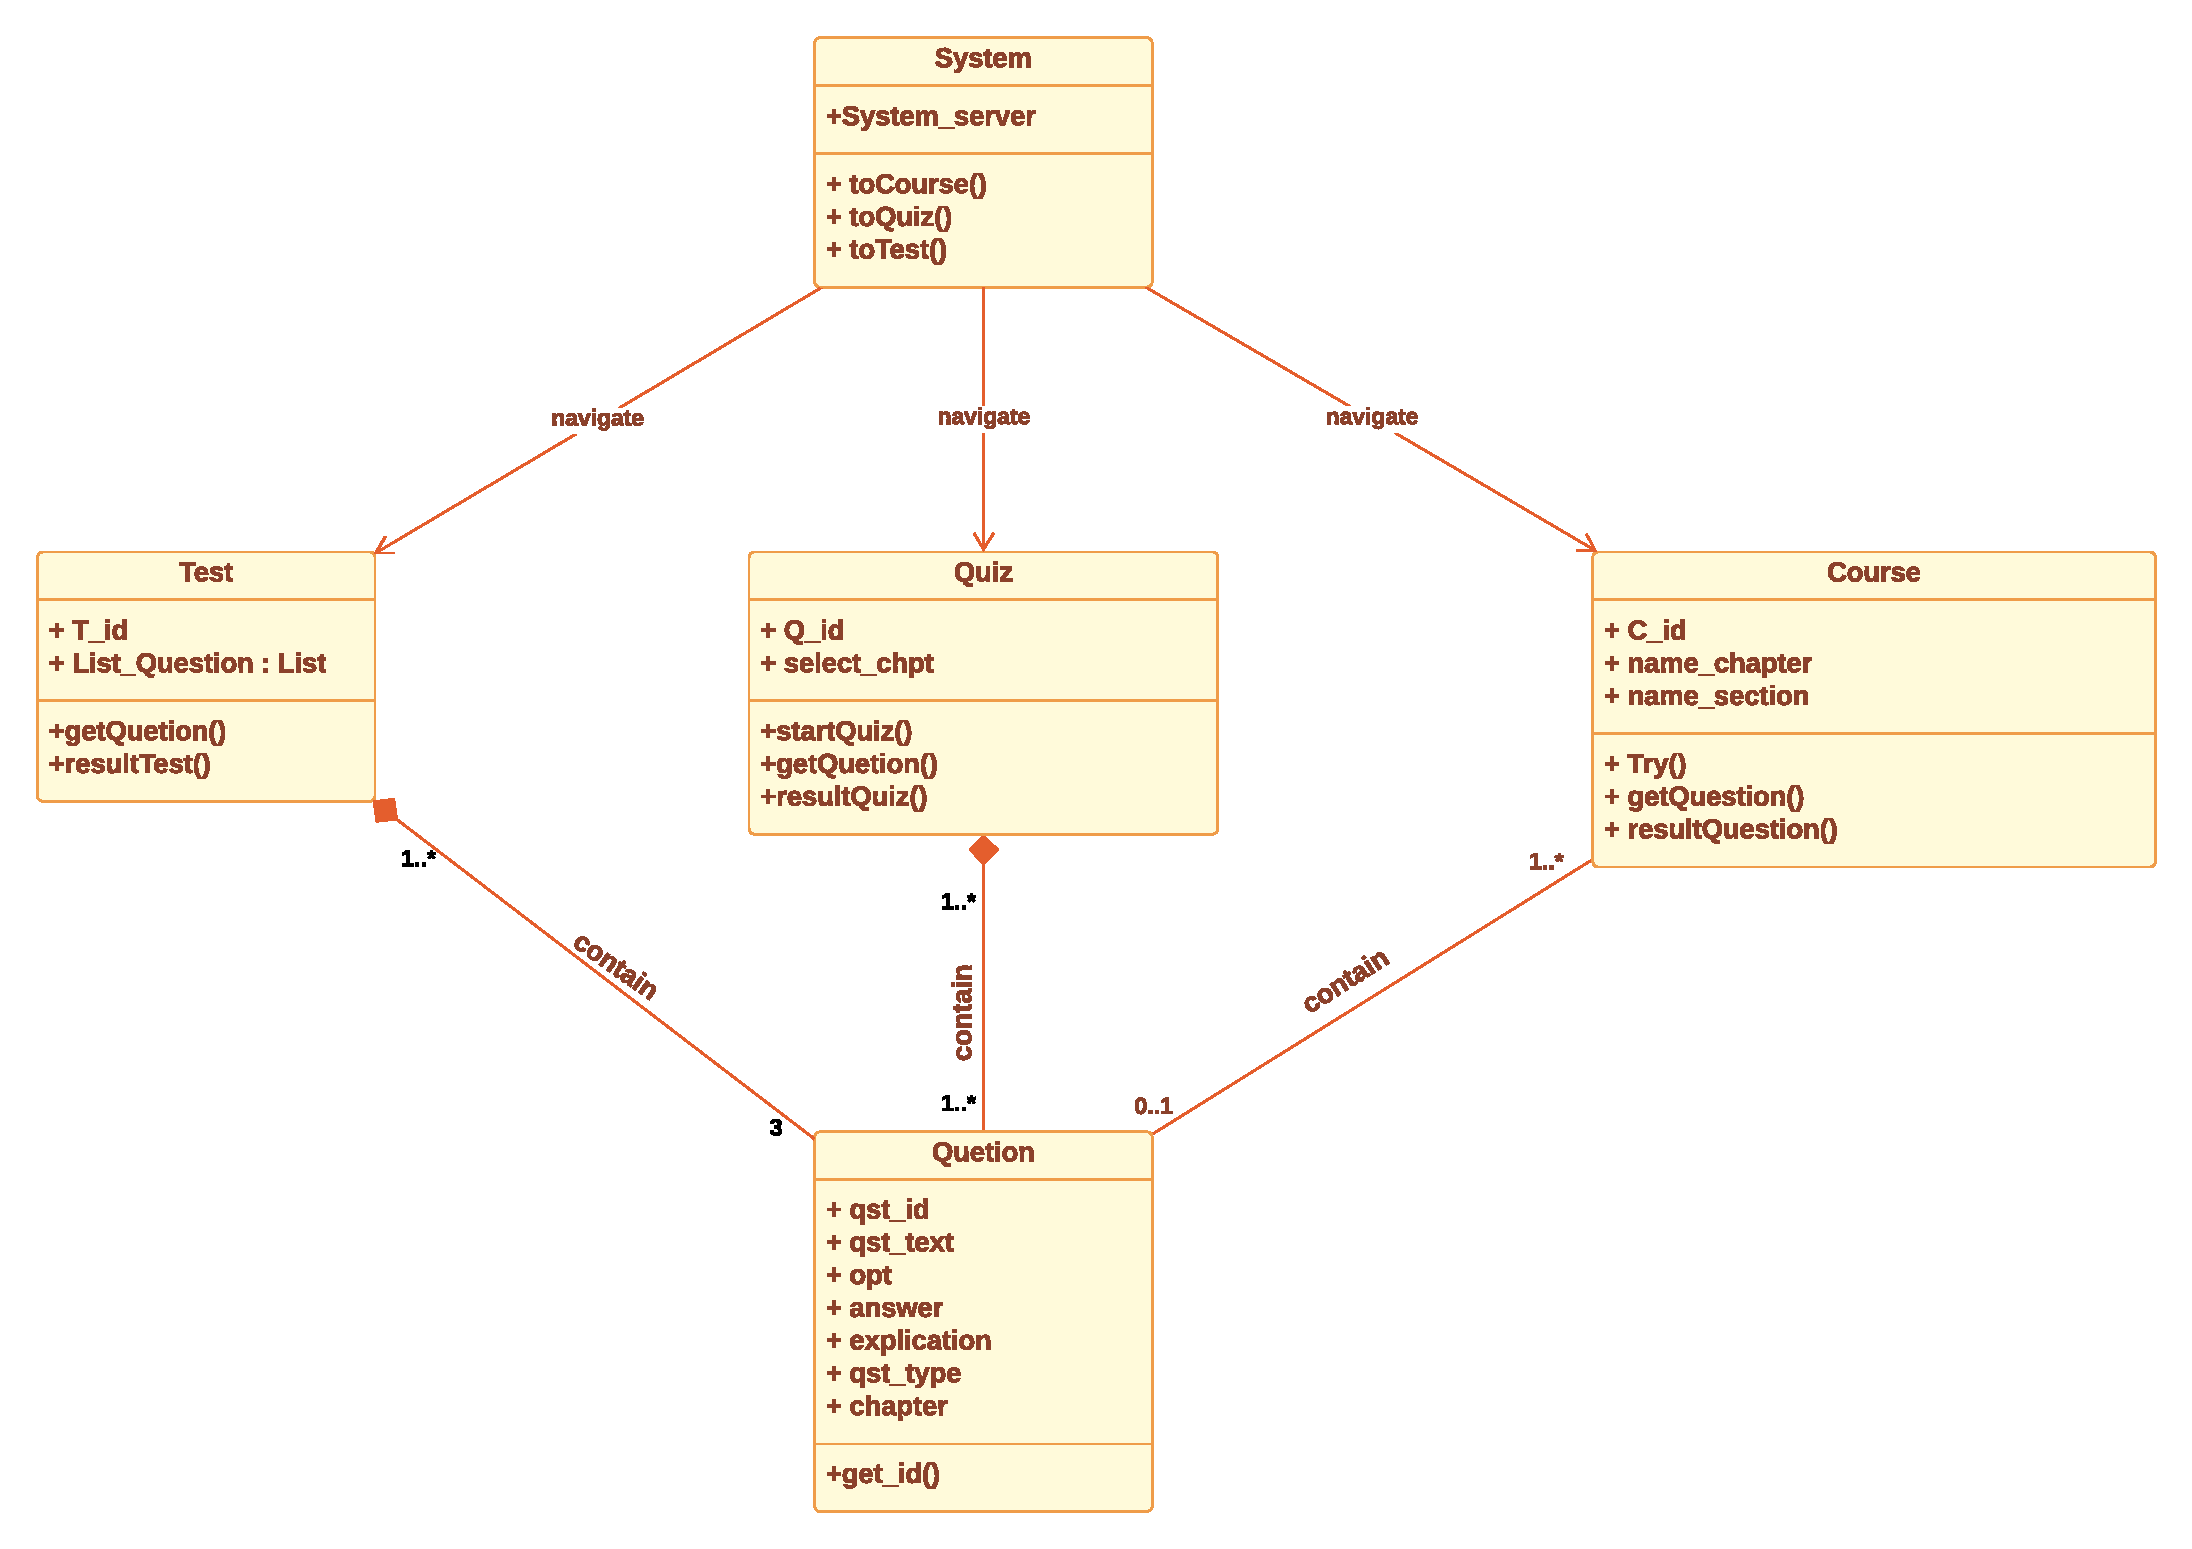
\includegraphics[scale=0.45]{img/UML class.pdf}                
	\caption{Class Diagram.} 
	\label{fig:DC}
\end{figure*} 
%===================================================================



\newpage
The table \ref{tab:DC} represents classes and attributes as well as their types and description .

\begin{table}[h!]
	\begin{center}
		\begin{tabular}{ |p{3cm}|p{3cm}|p{4cm}|p{2cm}|  }
 		\hline
 		Class & Attributes & Description & Type \\
 		\hline \hline
 		System & System-server & system's identificator. & Digital \\
 		\hline
 		Course & C-id & Course identificator. & Digital  \\
			& name-chapter & Chapter's name. & Alphabetic \\
			& name-title & Title's name. & Alphabetic \\
		\hline
		Quiz & Q-id & Quiz identificator. & Digital  \\
			& select-chpt & Choosing chapter. & Digital \\
			& nbr-qst & Number of questions. & Digital \\
		\hline
		Test & T-id & Test identificator. & Digital  \\
			& List-Question & List of questions. & Alphabetic \\
			& all-chpt & Choosing from all chapters. & Digital \\
		\hline
		Question & qst-id & Question identificator. & Digital  \\
			& nbr-qst & Number of questions. & Digital \\
			& select-chpt & Choosing chapter. & Digital \\
			& name-chapter & Chapter's name. & Alphabetic \\
			& name-title & Title's name. & Alphabetic \\
			& all-chpt & Choosing from all chapters. & Digital \\
		\hline
\end{tabular}
\end{center}
\caption{Description of Class Diagram.}
\label{tab:DC}
\end{table}


\newpage

\subsubsection{Database's Class Diagram}

The figure \ref{fig:BDD DC} represents the database in the form of a class diagram.\\\\\\

%***************************************************
\begin{figure*}[ht]
	\centering
	\label{}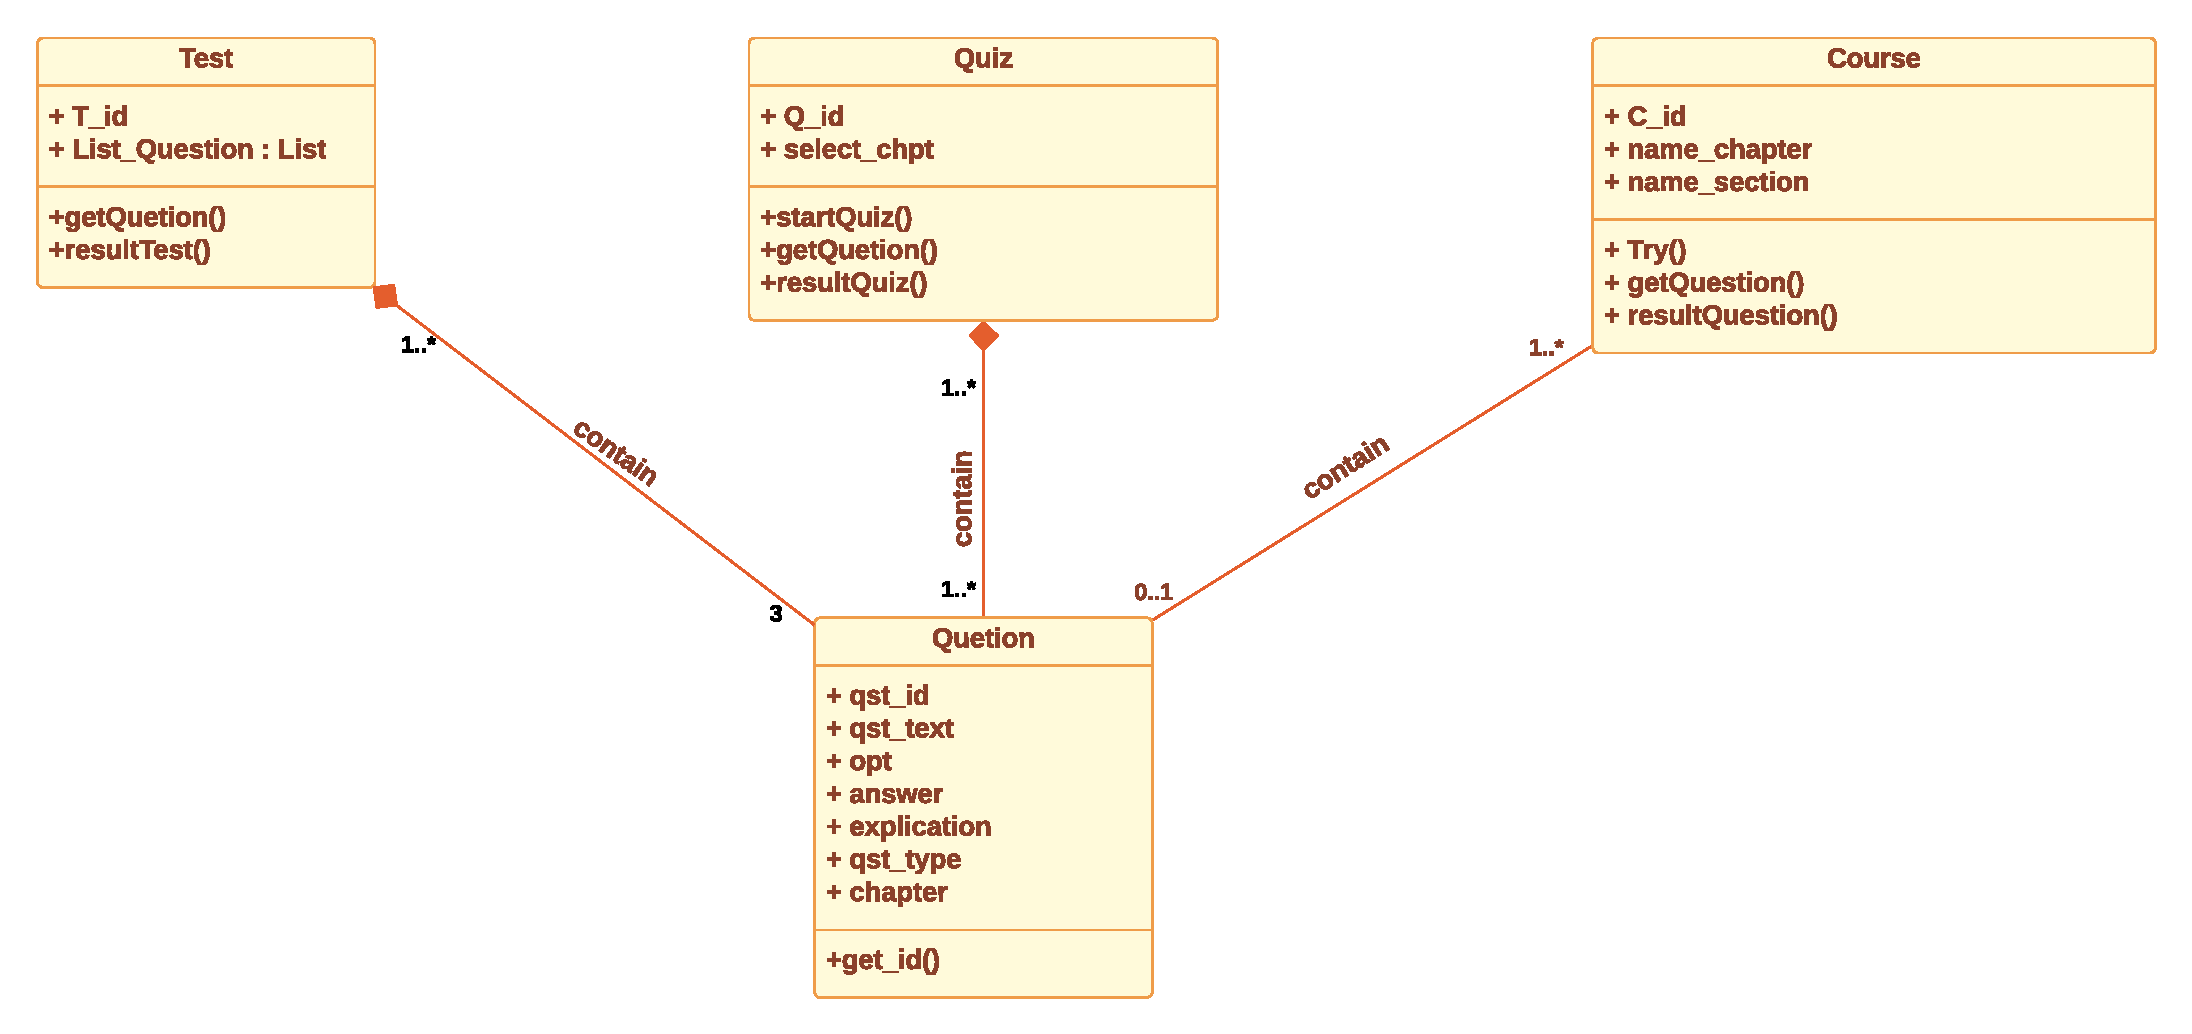
\includegraphics[scale=0.45]{img/BDD class.pdf}                
	\caption{Database's Class Diagram.} 
	\label{fig:BDD DC}
\end{figure*} 
%===================================================================



The table \ref{tab:BDD DC} represents classes and attributes of database's class diagram as well as their types and description.\\\\\\
\newpage
\begin{table}[h!]
	\begin{center}
		\begin{tabular}{ |p{3cm}|p{3cm}|p{4cm}|p{2cm}|  }
 		\hline
 		Class & attributes & Description & Type \\
 		\hline \hline
 		Course & C-id & Course identificator. & Digital  \\
			& name-chapter & Chapter's name. & Alphabetic \\
			& name-title & Title's name. & Alphabetic \\
		\hline
		Quiz & Q-id & Quiz identificator. & Digital  \\
			& select-chpt & Choosing chapter. & Digital \\
			& nbr-qst & Number of questions. & Digital \\
		\hline
		Test & T-id & Test identificator. & Digital  \\
			& List-Question & List of questions. & Alphabetic \\
			& all-chpt & Choosing from all chapters. & Digital \\
		\hline
		Question & qst-id & Question identificator. & Digital  \\
			& nbr-qst & Number of questions. & Digital \\
			& select-chpt & Choosing chapter. & Digital \\
			& name-chapter & Chapter's name. & Alphabetic \\
			& name-title & Title's name. & Alphabetic \\
			& all-chpt & Choosing from all chapters. & Digital \\
		\hline
\end{tabular}
\end{center}
\caption{Description of Database's Class Diagram.}
\label{tab:BDD DC}
\end{table}


\subsection{The relational model and creation of the Database}

A relational data model involves the use of data tables that collect groups of elements into relations. These models work based on the idea that each table setup will include a primary key or identifier. Other tables use that identifier to provide "relational" data links and results. Database administrators use something called Structured Query Language (SQL) to retrieve data elements from a relational database.\cite{Techopedia-relational-model} \\
Course(C-id,\#name-chapter,\#name-title).\\
Quiz(Q-id,\#select-chpt,\#nbr-qst).\\
Test(T-id,List-Question,\#all-chpt).\\
Question(qst-id,nbr-qst,select-chpt,name-chapter,name-title,all-chpt).\\


\section{Conclusion}
This chapter defined the basic steps for developing the system where specified functional and
non-functional requirements using the concepts of Unified Modeling Language ( Use Case
diagram, Sequence diagrams, and Class diagram), and clarified the goal of the analysis and
design. Next step is realizing the system
by introducing the programming languages, tools, and development environment used on
implementation.\\







